\subsection{Fiche d'avancement}

\newpage

\chapitre[
    $\mathbf{6^{\text{ème}}}$% : $\mathbf{6^{\text{ème}}}$,$\mathbf{5^{\text{ème}}}$,$\mathbf{4^{\text{ème}}}$,$\mathbf{3^{\text{ème}}}$,$\mathbf{2^{\text{nde}}}$,$\mathbf{1^{\text{ère}}}$,$\mathbf{T^{\text{Le}}}$,
    ]{
    % : ,Equations
    }{
    Collège% : Collège,Lycée
    }{
    Amadis Jamyn% : Amadis Jamyn,Eugène Belgrand
    }{
    % : ,\tableauPresenteEvalSixieme{}{10},\tableofcontents
    }{
        Fiche d'avancement% : Exercices
    }
\setcounter{tourcounter}{0}
\vspace{-0.8cm}\begin{center}
    \begin{tcbtab}{c|c|c|c|c}
        \'Equipe \no\repsim[1cm]{}& Joueur 1 & Joueur 2 & Joueur 3 & Joueur 4\\
        \hline
        Nom & \repsim[3.3cm]{} & \repsim[3.3cm]{} & \repsim[3.3cm]{} & \repsim[3.3cm]{}\\
        \hline
        Responsable de : & Dés & Fiche d'avancement & Curseur & Communication \\
    \end{tcbtab}
\end{center}
\vspace{-0.8cm}\begin{center}
    \begin{tcbtab}{c|c|c|c|c|c}
        %$\phantom{\dfrac{\dfrac{1}{10}}{\dfrac{1}{10}}}$ Tour $\phantom{\dfrac{\dfrac{1}{10}}{\dfrac{1}{10}}}$ & $1$ & $\dfrac{1}{10}$ & $\dfrac{1}{100}$ & Nombre formé & Résultat \\
        Action \no & Dé \no 1 & Dé \no 2 & Dé \no 3 & Nombre formé & Résultat \\
        \hline
        \repsim[1cm]{}  & \repsim{} & \repsim{} & \repsim{} & \repsim[3cm]{} & \repsim[6cm]{}\\
        \hline
        \repsim[1cm]{}  & \repsim{} & \repsim{} & \repsim{} & \repsim[3cm]{} & \repsim[6cm]{}\\
        \hline
        \repsim[1cm]{}  & \repsim{} & \repsim{} & \repsim{} & \repsim[3cm]{} & \repsim[6cm]{}\\
        \hline
        \repsim[1cm]{}  & \repsim{} & \repsim{} & \repsim{} & \repsim[3cm]{} & \repsim[6cm]{}\\
        \hline
        \repsim[1cm]{}  & \repsim{} & \repsim{} & \repsim{} & \repsim[3cm]{} & \repsim[6cm]{}\\
        \hline
        \repsim[1cm]{}  & \repsim{} & \repsim{} & \repsim{} & \repsim[3cm]{} & \repsim[6cm]{}\\
        \hline
        \repsim[1cm]{}  & \repsim{} & \repsim{} & \repsim{} & \repsim[3cm]{} & \repsim[6cm]{}\\
        \hline
        \repsim[1cm]{}  & \repsim{} & \repsim{} & \repsim{} & \repsim[3cm]{} & \repsim[6cm]{}\\
        \hline
        \repsim[1cm]{}  & \repsim{} & \repsim{} & \repsim{} & \repsim[3cm]{} & \repsim[6cm]{}\\
        \hline
        \repsim[1cm]{}  & \repsim{} & \repsim{} & \repsim{} & \repsim[3cm]{} & \repsim[6cm]{}\\
        \hline
        \repsim[1cm]{}  & \repsim{} & \repsim{} & \repsim{} & \repsim[3cm]{} & \repsim[6cm]{}\\
        \hline
        \repsim[1cm]{}  & \repsim{} & \repsim{} & \repsim{} & \repsim[3cm]{} & \repsim[6cm]{}\\
        \hline
        \repsim[1cm]{}  & \repsim{} & \repsim{} & \repsim{} & \repsim[3cm]{} & \repsim[6cm]{}\\
        \hline
        \repsim[1cm]{}  & \repsim{} & \repsim{} & \repsim{} & \repsim[3cm]{} & \repsim[6cm]{}\\
        \hline
        \repsim[1cm]{}  & \repsim{} & \repsim{} & \repsim{} & \repsim[3cm]{} & \repsim[6cm]{}\\
        \hline
        \repsim[1cm]{}  & \repsim{} & \repsim{} & \repsim{} & \repsim[3cm]{} & \repsim[6cm]{}\\
        \hline
        \repsim[1cm]{}  & \repsim{} & \repsim{} & \repsim{} & \repsim[3cm]{} & \repsim[6cm]{}\\
        \hline
        \repsim[1cm]{}  & \repsim{} & \repsim{} & \repsim{} & \repsim[3cm]{} & \repsim[6cm]{}\\
        \hline
        \repsim[1cm]{}  & \repsim{} & \repsim{} & \repsim{} & \repsim[3cm]{} & \repsim[6cm]{}\\
        \hline
        \repsim[1cm]{}  & \repsim{} & \repsim{} & \repsim{} & \repsim[3cm]{} & \repsim[6cm]{}
    \end{tcbtab}        
\end{center}

\newcommand{\drawGraduations}[3]{%
    % #1: Start value
    % #2: End value
    % #3: Offset value (for continuity)

    % Centièmes graduations (réduction du nombre de graduations)
    \def\scalefactor{1}

    \foreach \x in {#1,0.1,...,#2} {
        \draw[very thick] (0,\x*\scalefactor) -- (0.6, \x*\scalefactor);
    }

    % Dixièmes graduations
    \foreach \x in {#1,1,...,#2} {
        \draw[very thick] (0,\x*\scalefactor) -- (1.5, \x*\scalefactor);
    }

    % Unités graduations et affichage en grand et gras pour les entiers
    \foreach \x in {#1,1,...,\fpeval{#2+0.1}} {
        \draw[very thick] (0,\x*\scalefactor) -- (1.5, \x*\scalefactor);
        \pgfmathsetmacro{\value}{(\x + #3) / 10}
        \pgfmathsetmacro{\semivalue}{(\x + #3 + 5) / 10}
        \pgfmathsetmacro{\semiremainder}{mod(\semivalue,1)}
        \pgfmathsetmacro{\remainder}{mod(\value,1)}
        \ifdim \remainder pt = 0pt
            \node[left, font=\bfseries\LARGE] at (0, \x*\scalefactor) {\fpeval{\value}};
        \fi
        \ifdim \semiremainder pt = 0pt
            \node[left, font=\bfseries\large] at (0, \x*\scalefactor) {\num{\fpeval{\value}}};
        \fi
    }

        % Gamification : ajouter des événements aléatoires
        \pgfmathsetmacro{\randomShift}{rnd*4 - 2} % Générer une variation entre -2 et +2
        \pgfmathsetmacro{\eventCount}{int(5 + \randomShift)} % Base 5 événements avec une variation de -2 à +2
        \foreach \i in {1,...,\eventCount} {
        \pgfmathsetmacro{\randY}{random(\fpeval{#1},\fpeval{#2 - 3})}
        \pgfmathrandominteger{\randheight}{1}{2}
        \pgfmathsetmacro{\randX}{0.5*\bandwidth}
        \pgfmathrandominteger{\eventType}{1}{6}
        \def\eventcolor{yellow}
        \def\eventTextColor{black}
        % Définition des labels selon l'événement
        \ifnum\eventType=1
            \def\eventText{R}%Relancer les dés
            \def\eventcolor{green!85!black}
        \fi
        \ifnum\eventType=2
            \def\eventText{D}%Défi}
            \def\eventcolor{blue!35!white}
        \fi
        \ifnum\eventType=3
            \def\eventText{C}%Événement chanceux}
            \def\eventcolor{green!75!white}
        \fi
        \ifnum\eventType=4
            \def\eventText{D}%Défi}
            \def\eventcolor{blue!35!white}
        \fi
        \ifnum\eventType=5
            \def\eventText{M}%Événement malchanceux}
            \def\eventcolor{red!85!black}
            \def\eventTextColor{white}
        \fi
        \ifnum\eventType=6
            \def\eventText{D}%Défi}
            \def\eventcolor{blue!35!white}%green!75!white}
        \fi
        % Dessiner l'événement à une position aléatoire
        \draw[fill=\eventcolor, rounded corners] (\randX, \randY) rectangle ++(2, \randheight+1);

        % Calcul de l'intervalle et placement des labels
        \pgfmathsetmacro{\startY}{\randY}
        \pgfmathsetmacro{\endY}{\randY + \randheight}
        \foreach \y in {\startY, \fpeval{\startY + 1}, ..., \endY} {
            \node at (\randX + 1, \y + 0.5) {\LARGE{\textbf{\color{\eventTextColor}\eventText}}};
        }
    }
    
    % Languette de collage pour lier à la frise suivante
    \draw[thick, fill=gray!30] (0, \bandheight) rectangle (\bandwidth, \bandheight + \languette);
    \node[above, font=\small] at (\bandwidth/2, \bandheight + \languette / 10) {Languette de collage};
}





\subsection{Les curseurs}


\vspace{1.5cm}\begin{center}
    \curseur{blue}{1} \hspace{1cm} \curseur{red}{2} \hspace{1cm} \curseur{green}{3}
\end{center}

\vspace{1.5cm}\begin{center}
    \curseur{yellow}{4} \hspace{1cm} \curseur{purple}{5}
\end{center}

\subsection{Tutoriel}

\newpage

\def\bandwidth{4.5} % Largeur d'une bande en cm
\def\bandheight{25} % Hauteur d'une bande en cm
\def\languette{0.8}
\def\echellegraphique{10}
\def\nombremax{50}
\edef\nombrepage{\fpeval{round(\nombremax/(3*2.5),0)}}
\def\reste{1}
\newcommand{\drawTutoGraduations}[3]{%
    % #1: Start value
    % #2: End value
    % #3: Offset value (for continuity)

    % Centièmes graduations (réduction du nombre de graduations)
    \def\scalefactor{1}

    \foreach \x in {#1,0.1,...,#2} {
        \draw[very thick] (0,\x*\scalefactor) -- (0.6, \x*\scalefactor);
    }

    % Dixièmes graduations
    \foreach \x in {#1,1,...,#2} {
        \draw[very thick] (0,\x*\scalefactor) -- (1.5, \x*\scalefactor);
    }

    % Unités graduations et affichage en grand et gras pour les entiers
    \foreach \x in {#1,1,...,\fpeval{#2+0.1}} {
        \draw[very thick] (0,\x*\scalefactor) -- (1.5, \x*\scalefactor);
        \pgfmathsetmacro{\value}{(\x + #3) / 10}
        \pgfmathsetmacro{\semivalue}{(\x + #3 + 5) / 10}
        \pgfmathsetmacro{\semiremainder}{mod(\semivalue,1)}
        \pgfmathsetmacro{\remainder}{mod(\value,1)}
        \ifdim \remainder pt = 0pt
            \node[left, font=\bfseries\LARGE] at (0, \x*\scalefactor) {\fpeval{\value}};
        \fi
        \ifdim \semiremainder pt = 0pt
            \node[left, font=\bfseries\large] at (0, \x*\scalefactor) {\num{\fpeval{\value}}};
        \fi
    }

        % Gamification : ajouter des événements aléatoires
        \pgfmathsetmacro{\randomShift}{rnd*4 - 2} % Générer une variation entre -2 et +2
        \pgfmathsetmacro{\eventCount}{int(5 + \randomShift)} % Base 5 événements avec une variation de -2 à +2
        \foreach \i in {1,...,\eventCount} {
        \pgfmathsetmacro{\randY}{random(\fpeval{#1},\fpeval{#2 - 3})}
        \pgfmathrandominteger{\randheight}{1}{2}
        \pgfmathsetmacro{\randX}{0.5*\bandwidth}
        \pgfmathrandominteger{\eventType}{1}{6}
        \def\eventcolor{yellow}
        \def\eventTextColor{black}
        % Définition des labels selon l'événement
        \ifnum\eventType=1
            \def\eventText{R}%Relancer les dés
            \def\eventcolor{green!85!black}
        \fi
        \ifnum\eventType=2
            \def\eventText{M}%Événement malchanceux}
            \def\eventcolor{red!85!black}
            \def\eventTextColor{white}
        \fi
        \ifnum\eventType=3
            \def\eventText{C}%Événement chanceux}
            \def\eventcolor{green!75!white}
        \fi
        \ifnum\eventType=4
            \def\eventText{D}%Défi}
            \def\eventcolor{blue!35!white}
        \fi
        \ifnum\eventType=5
            \def\eventText{D}%Défi}
            \def\eventcolor{blue!35!white}
        \fi
        \ifnum\eventType=6
            \def\eventText{D}%Défi}
            \def\eventcolor{blue!35!white}%green!75!white}
        \fi
        % Dessiner l'événement à une position aléatoire
        \draw[fill=\eventcolor, rounded corners] (\randX, \randY) rectangle ++(2, \randheight+1);

        % Calcul de l'intervalle et placement des labels
        \pgfmathsetmacro{\startY}{\randY}
        \pgfmathsetmacro{\endY}{\randY + \randheight}
        \foreach \y in {\startY, \fpeval{\startY + 1}, ..., \endY} {
            \node at (\randX + 1, \y + 0.5) {\LARGE{\textbf{\color{\eventTextColor}\eventText}}};
        }
    }
    
    % Languette de collage pour lier à la frise suivante
    \draw[thick, fill=gray!30] (0, \bandheight) rectangle (\bandwidth, \bandheight + \languette);
    \node[above, font=\small] at (\bandwidth/2, \bandheight + \languette / 10) {Languette de collage};
}

% Votre commande de grille (adaptée ou existante)
\newcommand{\drawTutoGraduationsFixed}[4]{%
    % #1: valeur de début, #2: valeur de fin, #3: décalage numérique, #4: shift (position de la grille)
    \begin{scope}[shift={#4}]
        \def\scalefactor{1}
        
        % Tracé des graduations centièmes et dixièmes (exemple simplifié)
        \foreach \x in {#1,0.1,...,#2} {
            \draw[very thick] (0,\x*\scalefactor) -- (0.6,\x*\scalefactor);
        }
        \foreach \x in {#1,1,...,#2} {
            \draw[very thick] (0,\x*\scalefactor) -- (1.5,\x*\scalefactor);
        }
        % Unités graduations et affichage en grand et gras pour les entiers
        \foreach \x in {#1,1,...,\fpeval{#2+0.1}} {
            \draw[very thick] (0,\x*\scalefactor) -- (1.5, \x*\scalefactor);
            \pgfmathsetmacro{\value}{(\x + #3) / 10}
            \pgfmathsetmacro{\semivalue}{(\x + #3 + 5) / 10}
            \pgfmathsetmacro{\semiremainder}{mod(\semivalue,1)}
            \pgfmathsetmacro{\remainder}{mod(\value,1)}
            \ifdim \remainder pt = 0pt
                \node[left, font=\bfseries\LARGE] at (0, \x*\scalefactor) {\fpeval{\value}};
            \fi
            \ifdim \semiremainder pt = 0pt
                \node[left, font=\bfseries\large] at (0, \x*\scalefactor) {\num{\fpeval{\value}}};
            \fi
        }
    \end{scope}
}

% Commande pour dessiner les événements fixes sur la frise
\newcommand{\drawFixedEvents}{%
  \def\eventx{0.5*\bandwidth}%
  % Événement 1 : Défi (9 à 11)
  \draw[fill=blue!35, rounded corners] (\eventx,10) rectangle ++(2,2);
  \node at ($(\eventx,10)!0.5!(\eventx+2,12)$) {\LARGE \textbf{D}};
  % Événement 2 : Chanceux (12 à 13)
  \draw[fill=green!75!white, rounded corners] (\eventx,12) rectangle ++(2,1);
  \node at ($(\eventx,12)!0.5!(\eventx+2,13)$) {\LARGE \textbf{C}};
  % Événement 3 : Autre défi (15 à 17)
  \draw[fill=blue!35, rounded corners] (\eventx,15) rectangle ++(2,2);
  \node at ($(\eventx,15)!0.5!(\eventx+2,17)$) {\LARGE \textbf{D}};
  % Événement 4 : Malchanceux (21 à 23)
  \draw[fill=red!85!black, rounded corners] (\eventx,21) rectangle ++(2,2);
  \node at ($(\eventx,21)!0.5!(\eventx+2,23)$) {\LARGE \textbf{\color{white}M}};
  % Événement 5 : Relance (28 à 31)
  \draw[fill=green!85!black, rounded corners] (\eventx,28) rectangle ++(2,3);
  \node at ($(\eventx,28)!0.5!(\eventx+2,31)$) {\LARGE \textbf{R}};
}


\newcommand{\placecurseurAt}[4]{%
    % #1 : Couleur du curseur
    % #2 : Numéro de l'équipe
    % #3 : Coordonnée x
    % #4 : Coordonnée y
    \begin{scope}[shift={(#3,#4)}]
         % Flèche tournée vers la droite (miroir de celle d'origine)
         \fill[#1] (2,0) -- (0,1) -- (0.5,0) -- (0,-1) -- cycle;
         \draw[thick, black] (2,0) -- (0,1) -- (0.5,0) -- (0,-1) -- cycle;
         
         % Bulle (positionnée à gauche de la flèche)
         \fill[#1!50] (-0.5,0) circle (1);
         \draw[thick, black] (-0.5,0) circle (1);
         
         % Queue reliant la bulle (placée sur le côté droit de la bulle)
         \fill[#1!50] (0,0) -- (-0.2,-0.2) -- (-0.4,0.1) -- cycle;
         
         % Texte dans la bulle
         \node at (-0.5,0) {\textbf{\Huge #2}};

         % Position pour le tuto
         \draw[line width=2pt, #1!65!black, dashed] (2,0) -- (2+\bandwidth,0);

         % abscisse du curseur
         \node at (3+\bandwidth,0) {\color{#1!85!black} \Huge $\mathbf{\num{\fpeval{#4 / 10}}}$};
    \end{scope}
}
\newcommand{\flechedeplacement}[3]{%
  \begin{scope}
    % Paramètres de la flèche
    \def\arrowThickness{0.6} % épaisseur de la flèche en cm
    \def\arrowHead{0.5}      % hauteur de la pointe en cm
    
    % Calcul de la moitié de l'épaisseur pour centrer la flèche sur l'axe horizontal
    \pgfmathsetmacro{\halfThickness}{\arrowThickness/2}%
    % Position horizontale centrée sur la frise (en supposant que \bandwidth est défini)
    \pgfmathsetmacro{\xcenter}{\bandwidth/2}%
    % Position pour le tuto
    \draw[line width=2pt, #1!65!black, dashed] (0,#2) -- (\bandwidth,#2);

    % abscisse du curseur
    \node at (1 +\bandwidth,#2) {\color{#1!85!black} \Huge $\mathbf{\num{\fpeval{#2 / 10}}}$};
    % distance parcourue
    \pgfmathsetmacro{\ycoord}{(#2+#3)/2}%
    \node at (2+\bandwidth,\ycoord) {\color{#1!85!black} \Huge $\mathbf{+\num{\fpeval{(#3 - #2)/10}}}$};
    
    % Dessin de la flèche (forme de polygone)
    \filldraw[fill={#1!50!white}, draw=black, line width=1pt]
         (\xcenter - \halfThickness, #2) --
         (\xcenter + \halfThickness, #2) --
         (\xcenter + \halfThickness, {#3 - \arrowHead}) --
         (\xcenter, #3) --
         (\xcenter - \halfThickness, {#3 - \arrowHead}) -- cycle;
  \end{scope}%
}
\newcommand{\flecherecul}[3]{%
  \begin{scope}
    % Paramètres de la flèche
    \def\arrowThickness{0.6} % épaisseur de la flèche en cm
    \def\arrowHead{0.5}      % hauteur de la pointe en cm
    
    % Calcul de la moitié de l'épaisseur (pour centrer la flèche horizontalement)
    \pgfmathsetmacro{\halfThickness}{\arrowThickness/2}%
    % Position horizontale centrée sur la frise (on suppose que \bandwidth est défini)
    \pgfmathsetmacro{\xcenter}{\bandwidth/2}%
    % Position pour la ligne horizontale ( départ )
    \draw[line width=2pt, #1!65!black, dashed] (0,#2) -- (\bandwidth,#2);
    % abscisse du départ
    \node at (1+\bandwidth,#2) {\color{#1!85!black} \Huge $\mathbf{\num{\fpeval{#2 / 10}}}$};
    % distance parcourue
    \pgfmathsetmacro{\ycoord}{(#2+#3)/2}%
    \node at (2+\bandwidth,\ycoord) {\color{#1!85!black} \Huge $\mathbf{-\num{\fpeval{(#2 - #3)/10}}}$};
        % Construction de la flèche inversée (point en bas)
    \filldraw[fill={#1!50!white}, draw=black, line width=1pt]
         % Partie supérieure du rectangle
         (\xcenter - \halfThickness - 0.5, #2) --  % coin supérieur gauche
         (\xcenter + \halfThickness - 0.5, #2) --  % coin supérieur droit
         % Descente du rectangle jusqu'au début de la pointe
         (\xcenter + \halfThickness - 0.5, {#3 + \arrowHead}) -- 
         % Pointe : le sommet de la flèche (centre en bas)
         (\xcenter - 0.5, #3) -- 
         % Retour par le côté gauche
         (\xcenter - \halfThickness - 0.5, {#3 + \arrowHead}) -- 
         cycle;
  \end{scope}%
}

\begin{multicols}{2}
\begin{tikzpicture}[x=1cm, y=1cm,xshift=-0.5cm,yshift=0.5cm]

    % Dessin de la première bande
    \begin{scope}[shift={(2,1)}]
        \draw[thick] (0,0) rectangle (\bandwidth, \bandheight);
        \clip (-4,-1) rectangle (\bandwidth + 4, \bandheight+\languette+1);
        %\drawTutoGraduations{0}{25}{0}
        % Exemple d'utilisation de la commande de grille
        \drawTutoGraduationsFixed{0}{25}{0}{(0,0)}
        % Ajout des événements fixes sur la frise
        \drawFixedEvents
        \placecurseurAt{blue}{1}{-2}{10.7}
        \placecurseurAt{red}{2}{-2}{0}
        \flechedeplacement{blue}{0}{10.7}%{15}
        %\placecurseurAt{green}{3}{-2}{23}
    \end{scope}
    
    
\end{tikzpicture}

\columnbreak

\phantom{a}
\vfill
\begin{center}
    \begin{minipage}{0.7\columnwidth}
    \boite{Action \no 1 :}{
        \begin{enumerate}
            \item L'équipe \no 1 lance les dés et obtient $1$ ; $0$ et $7$.
            \item Le responsable remplit la fiche d'avancement en \acc{composant} le nombre $\num{1.07}$. 
            \item Le responsable du curseur le place sur la frise.
            \item Le responsable de la communication annonce \frquote{Pour contrôle !}
            \item L'équipe d'arbitrage valide la position.
        \end{enumerate}
    }
    \end{minipage}
\end{center}
\vfill
\phantom{a}
\end{multicols}


\newpage

\begin{multicols}{2}
    \begin{tikzpicture}[x=1cm, y=1cm,xshift=-0.5cm,yshift=0.5cm]
    
        % Dessin de la première bande
        \begin{scope}[shift={(2,1)}]
            \draw[thick] (0,0) rectangle (\bandwidth, \bandheight);
            \clip (-4,-1) rectangle (\bandwidth + 4, \bandheight+\languette+1);
            %\drawTutoGraduations{0}{25}{0}
            % Exemple d'utilisation de la commande de grille
            \drawTutoGraduationsFixed{0}{25}{0}{(0,0)}
            % Ajout des événements fixes sur la frise
            \drawFixedEvents
            \placecurseurAt{blue}{1}{-2}{20.7}
            \placecurseurAt{red}{2}{-2}{0}
            \flechedeplacement{blue}{10.7}{20.7}%\placecurseurAt{green}{3}{-2}{23}
        \end{scope}
        
        
    \end{tikzpicture}
    
    \columnbreak
    
    \phantom{a}
    \vfill
    \begin{center}
        \begin{minipage}{0.7\columnwidth}
            \boite{Action \no 2 :}{
                \begin{enumerate}
                    \item L'équipe \no 1 se trouve sur une case \frquote{Défi} : elle pioche un problème.
                    \item Elle obtient le problème de niveau 1 suivant et donne la bonne réponse.\\
                    
                    \mesTutocartes{green}{Q.1.3}{ $17+25$ }{S.1.3}{$17+25=42$}%
    
                    \item L'équipe d'arbitrage valide la réponse.
                    \item Le responsable du curseur avance d'une unité.
                    \item Le responsable de la communication annonce \frquote{Pour contrôle !}
                    \item L'équipe d'arbitrage valide la position.
                \end{enumerate}
            }
        \end{minipage}
    \end{center}
    \vfill
    \phantom{a}
    \end{multicols}
    
    
    \newpage

    \begin{multicols}{2}
        \begin{tikzpicture}[x=1cm, y=1cm,xshift=-0.5cm,yshift=0.5cm]
        
            % Dessin de la première bande
            \begin{scope}[shift={(2,1)}]
                \draw[thick] (0,0) rectangle (\bandwidth, \bandheight);
                \clip (-4,-1) rectangle (\bandwidth + 4, \bandheight+\languette+1);
                %\drawTutoGraduations{0}{25}{0}
                % Exemple d'utilisation de la commande de grille
                \drawTutoGraduationsFixed{0}{25}{0}{(0,0)}
                % Ajout des événements fixes sur la frise
                \drawFixedEvents
                \placecurseurAt{blue}{1}{-2}{20.7}
                \placecurseurAt{red}{2}{-2}{18.4}
                %\placecurseurAt{green}{3}{-2}{23}
                \flechedeplacement{red}{0}{18.4}
            \end{scope}
            
            
        \end{tikzpicture}
        
        \columnbreak
        
        \phantom{a}
        \vfill
        \begin{center}
            \begin{minipage}{0.7\columnwidth}
            \boite{Action \no 3 :}{
                \begin{enumerate}
                    \item L'équipe \no 2 lance les dés et obtient $1$ ; $8$ et $4$.
                    \item Le responsable complète la fiche d'avancement.    
                    \item Le responsable du curseur le place sur la frise.
                    \item Le responsable de la communication annonce \frquote{Pour contrôle !}
                    \item L'équipe d'arbitrage valide la position.
                \end{enumerate}
            }
            \end{minipage}
        \end{center}
        \vfill
        \phantom{a}
        \end{multicols}

\newpage

\begin{multicols}{2}
    \begin{tikzpicture}[x=1cm, y=1cm,xshift=-0.5cm,yshift=0.5cm]
    
        % Dessin de la première bande
        \begin{scope}[shift={(2,1)}]
            \draw[thick] (0,0) rectangle (\bandwidth, \bandheight);
            \clip (-4,-1) rectangle (\bandwidth + 4, \bandheight+\languette+1);
            %\drawTutoGraduations{0}{25}{0}
            % Exemple d'utilisation de la commande de grille
            \drawTutoGraduationsFixed{0}{25}{0}{(0,0)}
            % Ajout des événements fixes sur la frise
            \drawFixedEvents
            \placecurseurAt{blue}{1}{-2}{22.8}
            \placecurseurAt{red}{2}{-2}{18.4}
            %\placecurseurAt{green}{3}{-2}{23}
            \flechedeplacement{blue}{20.7}{22.8}
        \end{scope}
        
        
    \end{tikzpicture}
    
    \columnbreak
    
    \phantom{a}
    \vfill
    \begin{center}
        \begin{minipage}{0.7\columnwidth}
        \boite{Action \no 4 :}{
            \begin{enumerate}
                \item L'équipe \no 1 lance les dés et obtient $0$ ; $2$ et $1$.
                \item Le responsable complète la fiche d'avancement :
                
                $\num{2.07} + \num{0.21} = \num{\fpeval{2.07+0.21}}$
                \item Le responsable du curseur le place sur la frise.
                \item Le responsable de la communication annonce \frquote{Pour contrôle !}
                \item L'équipe d'arbitrage valide la position.
            \end{enumerate}
        }
        \end{minipage}
    \end{center}
    \vfill
    \phantom{a}
    \end{multicols}

\newpage

\begin{multicols}{2}
    \begin{tikzpicture}[x=1cm, y=1cm,xshift=-0.5cm,yshift=0.5cm]
    
        % Dessin de la première bande
        \begin{scope}[shift={(2,1)}]
            \draw[thick] (0,0) rectangle (\bandwidth, \bandheight);
            \clip (-4,-1) rectangle (\bandwidth + 4, \bandheight+\languette+1);
            %\drawTutoGraduations{0}{25}{0}
            % Exemple d'utilisation de la commande de grille
            \drawTutoGraduationsFixed{0}{25}{0}{(0,0)}
            % Ajout des événements fixes sur la frise
            \drawFixedEvents
            \placecurseurAt{blue}{1}{-2}{12.8}
            \placecurseurAt{red}{2}{-2}{18.4}
            %\placecurseurAt{green}{3}{-2}{23}
            \flecherecul{blue}{22.8}{12.8}
        \end{scope}
        
        
    \end{tikzpicture}
    
    \columnbreak
    
    \phantom{a}
    \vfill
    \begin{center}
        \begin{minipage}{0.7\columnwidth}
        \boite{Action \no 5 :}{
            \begin{enumerate}
                \item L'équipe \no 1 \acc{recule} d'une unité puisque le curseur atterit sur une case \frquote{Malchance}.
                \item Le responsable complète la fiche d'avancement.    
                \item Le responsable du curseur le place sur la frise.
                \item Le responsable de la communication annonce \frquote{Pour contrôle !}
                \item L'équipe d'arbitrage valide la position.
                \item Même si l'équipe arrive sur un événement \frquote{Chanceux}, elle ne le déclenche pas car elle a déjà eu un événement ce tour. 
            \end{enumerate}
        }
        \end{minipage}
    \end{center}
    \vfill
    \phantom{a}
    \end{multicols}

\newpage



\newpage

\subsection{La frise}

\newpage

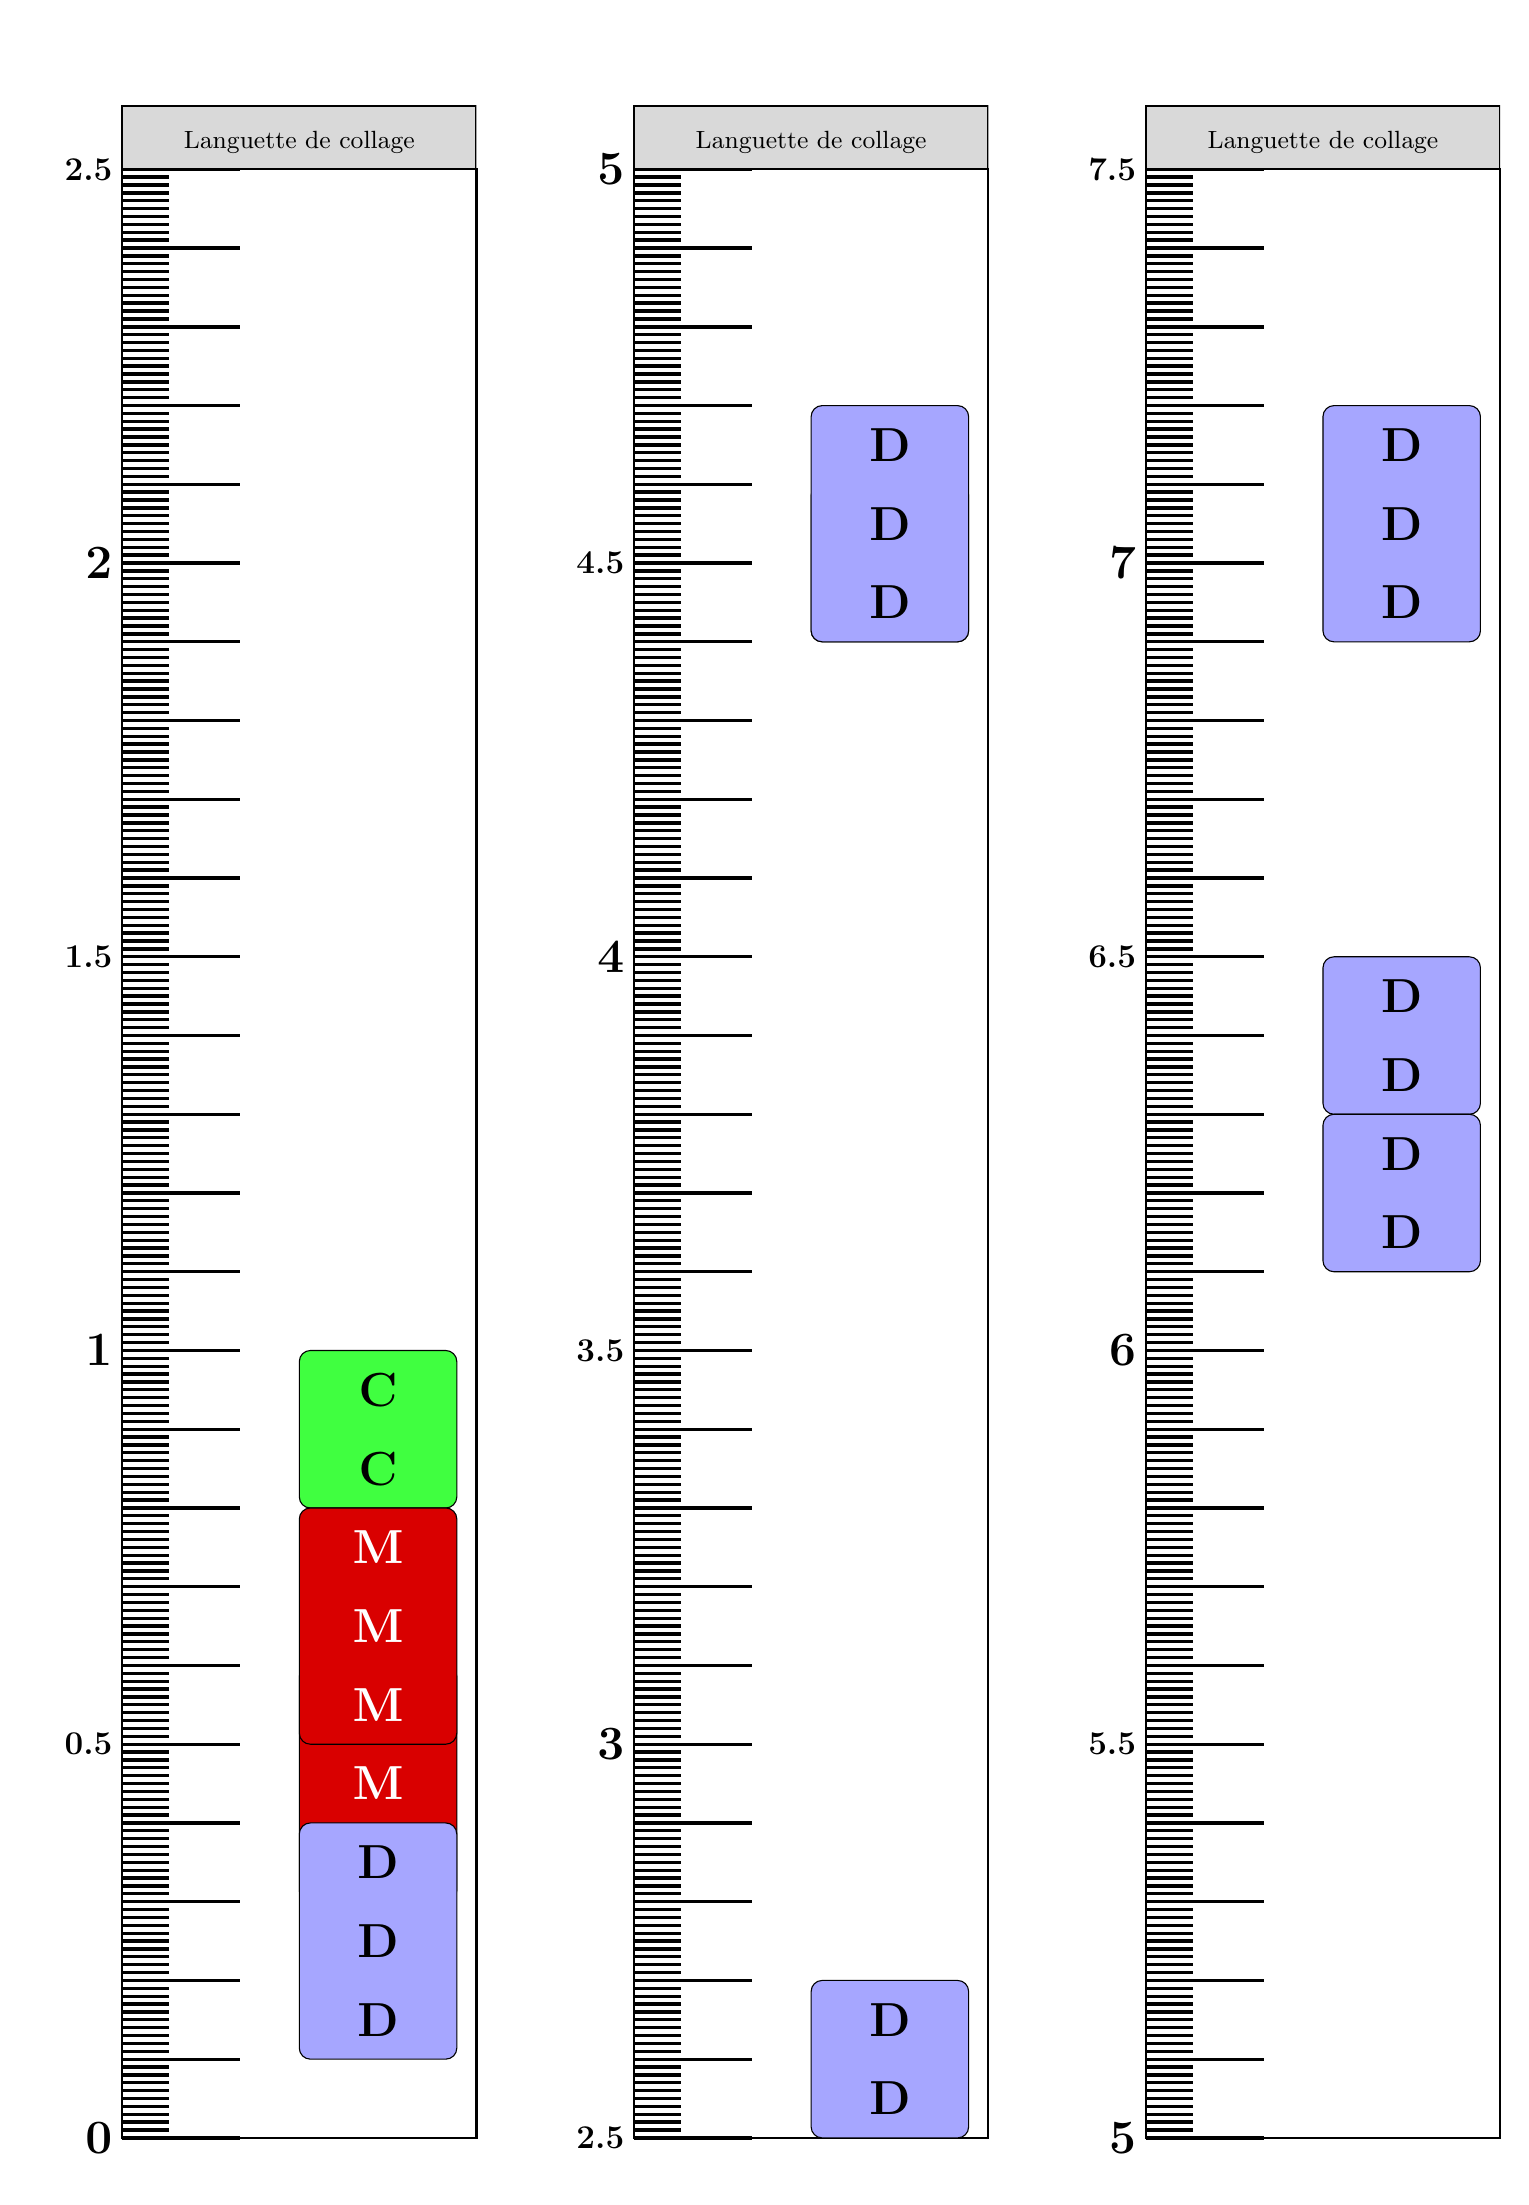
\begin{tikzpicture}[x=1cm, y=1cm,xshift=-1cm]

% Dessin de la première bande
\begin{scope}[shift={(-1,0)}]
    \draw[thick] (0,0) rectangle (\bandwidth, \bandheight);
    \clip (-1.2,-0.5) rectangle (\bandwidth, \bandheight+\languette+1);
    \drawGraduations{0}{25}{0}
\end{scope}

% Dessin de la deuxième bande (avec continuité des nombres)
\begin{scope}[shift={(1*\bandwidth + 1,0)}]
    \draw[thick] (0,0) rectangle (\bandwidth, \bandheight);
    \clip (-1.2,-0.5) rectangle (\bandwidth, \bandheight+\languette+1);
    \drawGraduations{0}{25}{25}
\end{scope}

% Dessin de la troisième bande (avec continuité des nombres)
\begin{scope}[shift={(2*\bandwidth + 3,0)}]
    \draw[thick] (0,0) rectangle (\bandwidth, \bandheight);
    \clip (-1.2,-0.5) rectangle (\bandwidth, \bandheight+\languette+1);
    \drawGraduations{0}{25}{50}
\end{scope}

\end{tikzpicture}

\newpage

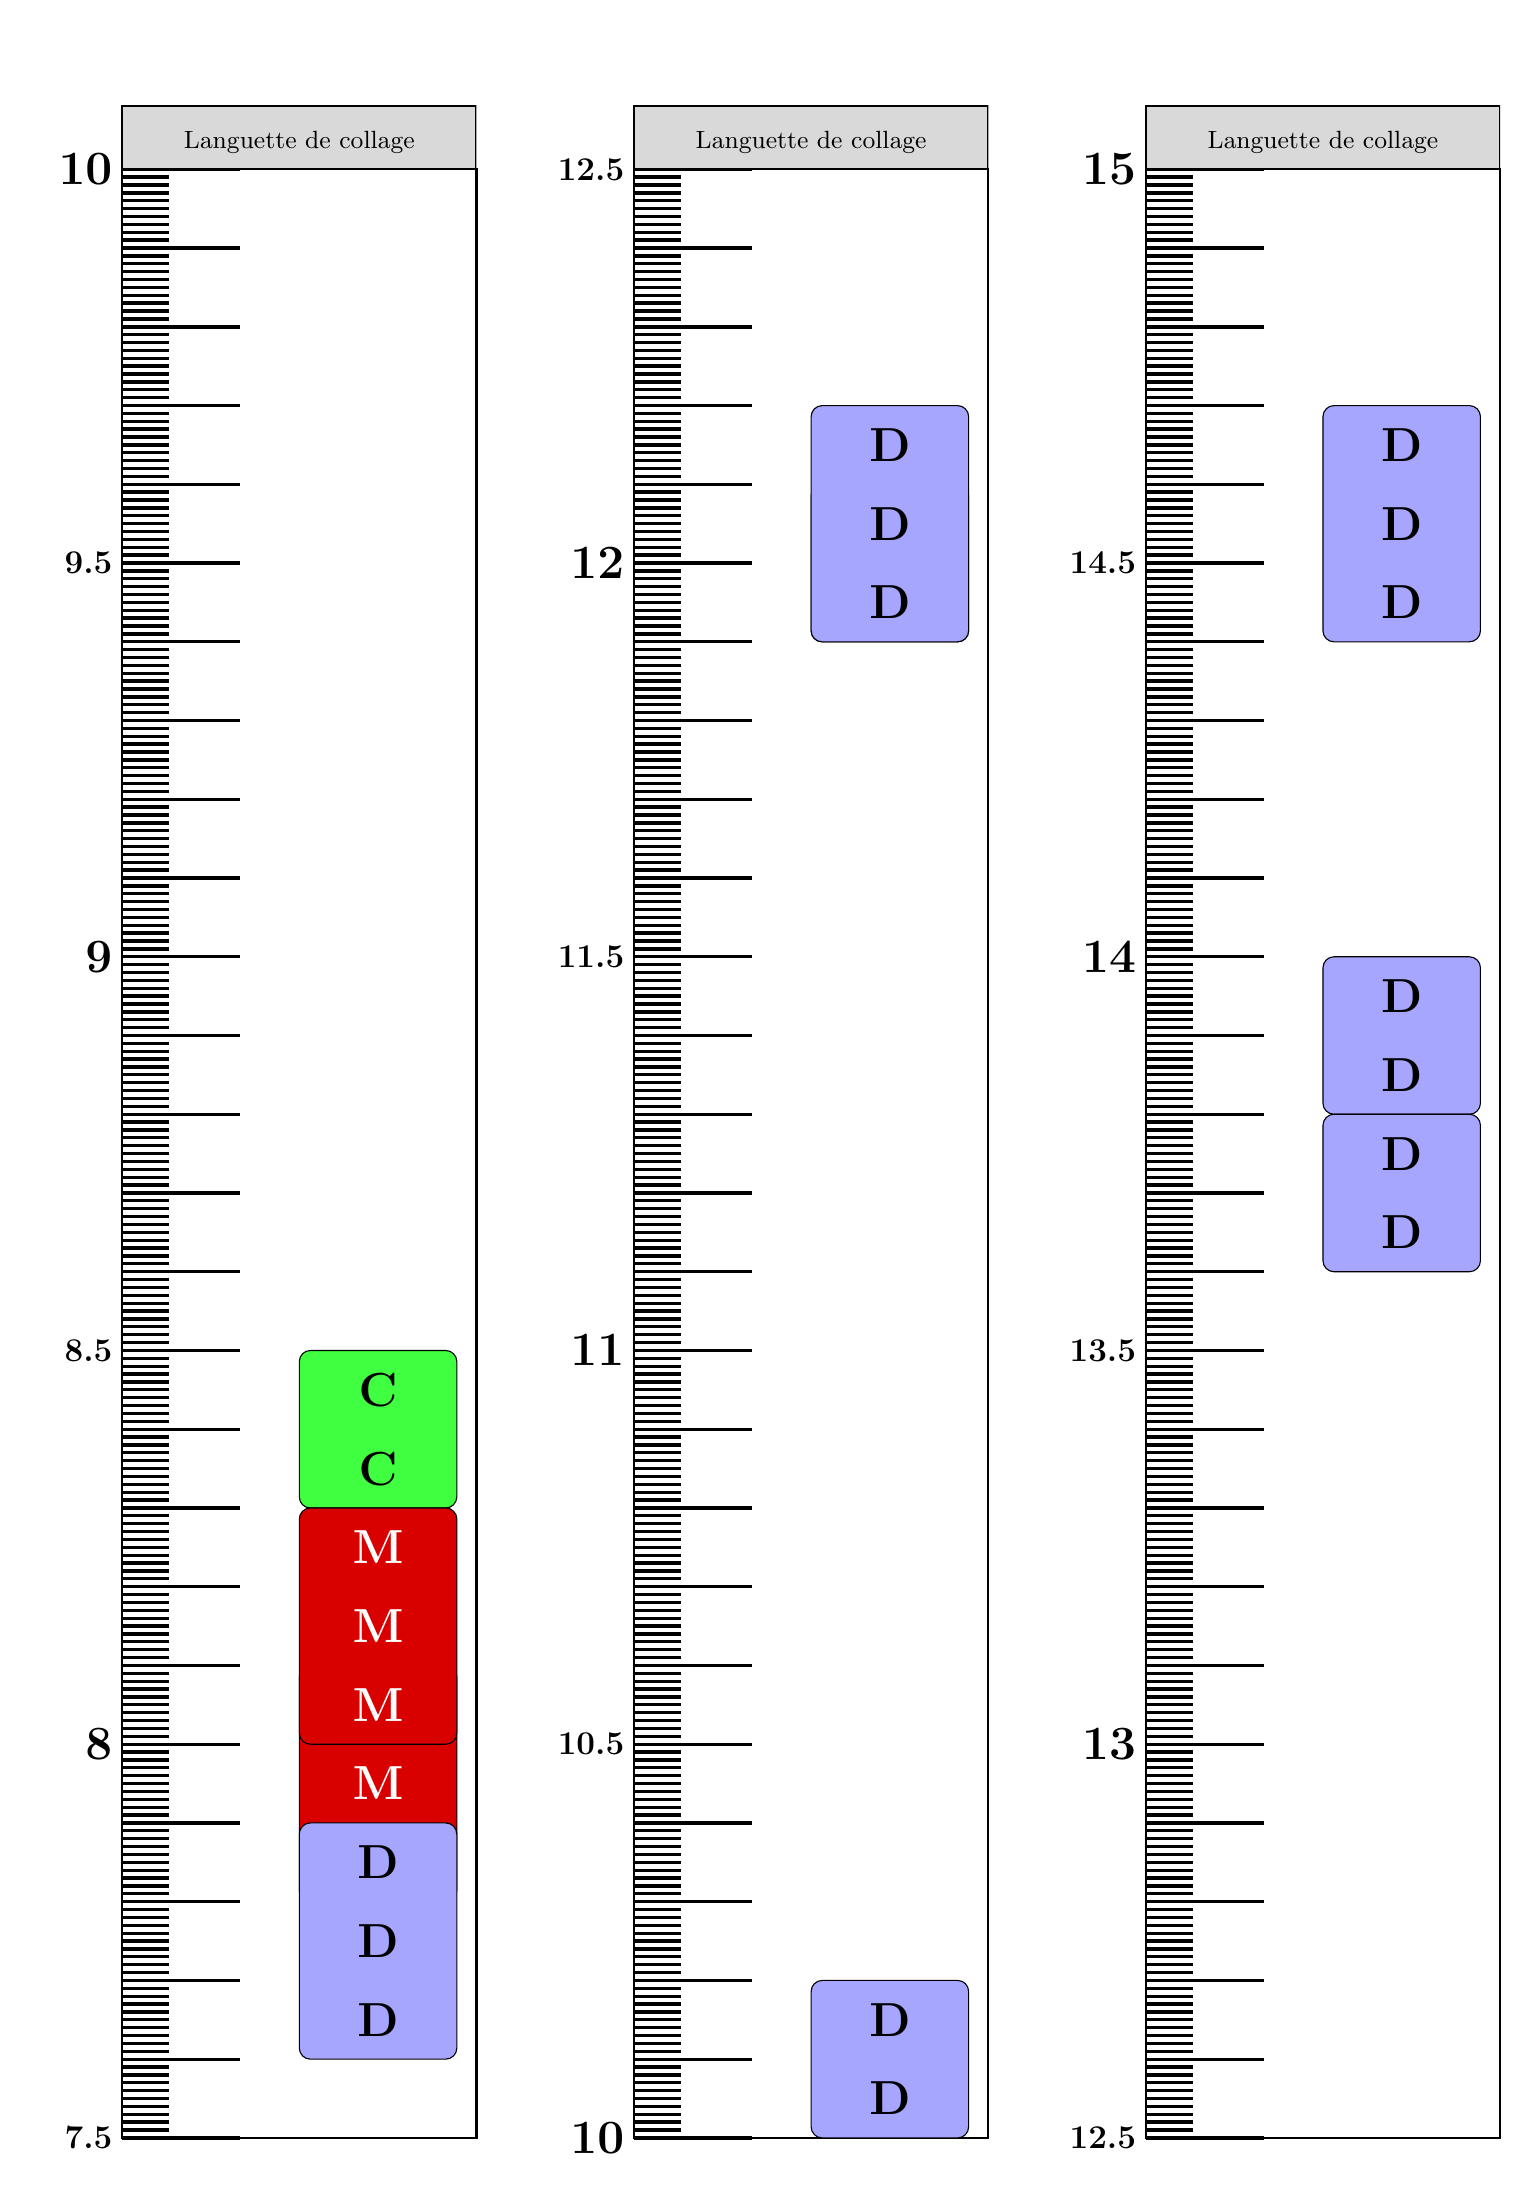
\begin{tikzpicture}[x=1cm, y=1cm,xshift=-1cm]
% Dessin de la première bande
\begin{scope}[shift={(-1,0)}]
    \draw[thick] (0,0) rectangle (\bandwidth, \bandheight);
    \clip (-1.2,-0.5) rectangle (\bandwidth, \bandheight+\languette+1);
    \drawGraduations{0}{25}{75}
\end{scope}

% Dessin de la deuxième bande (avec continuité des nombres)
\begin{scope}[shift={(1*\bandwidth + 1,0)}]
    \draw[thick] (0,0) rectangle (\bandwidth, \bandheight);
    \clip (-1.2,-0.5) rectangle (\bandwidth, \bandheight+\languette+1);
    \drawGraduations{0}{25}{100}
\end{scope}

% Dessin de la troisième bande (avec continuité des nombres)
\begin{scope}[shift={(2*\bandwidth + 3,0)}]
    \draw[thick] (0,0) rectangle (\bandwidth, \bandheight);
    \clip (-1.2,-0.5) rectangle (\bandwidth, \bandheight+\languette+1);
    \drawGraduations{0}{25}{125}
\end{scope}

\end{tikzpicture}

\newpage

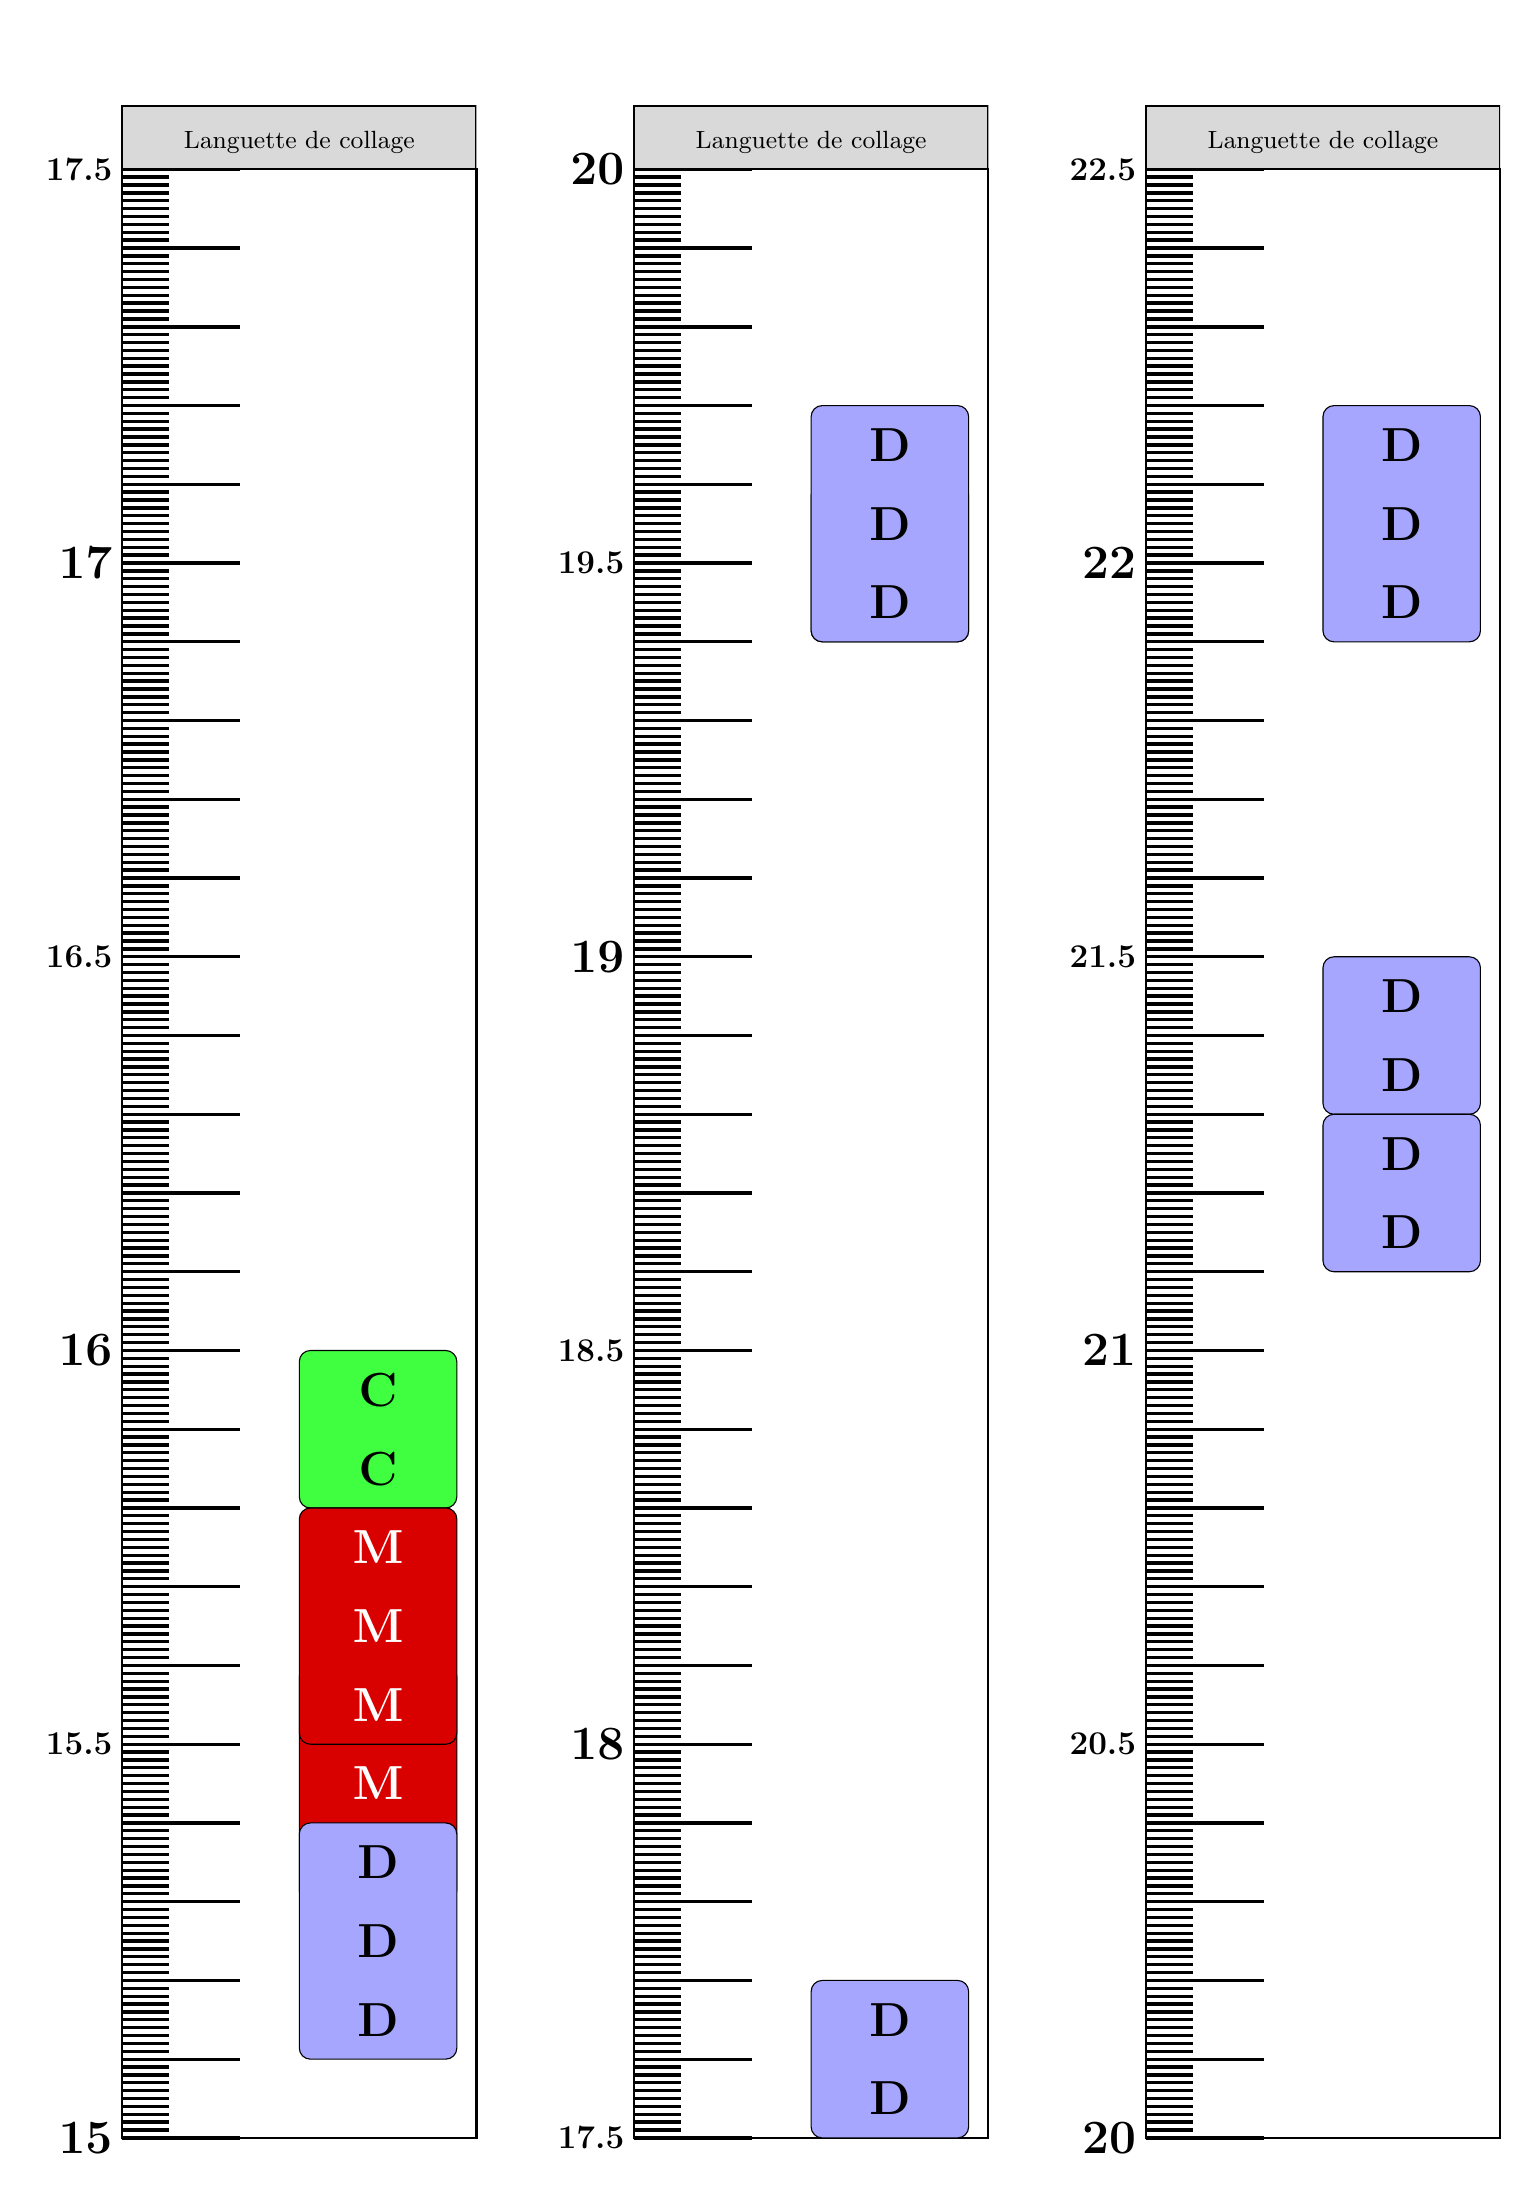
\begin{tikzpicture}[x=1cm, y=1cm,xshift=-1cm]
% Dessin de la première bande
\begin{scope}[shift={(-1,0)}]
    \draw[thick] (0,0) rectangle (\bandwidth, \bandheight);
    \clip (-1.2,-0.5) rectangle (\bandwidth, \bandheight+\languette+1);
    \drawGraduations{0}{25}{150}
\end{scope}

% Dessin de la deuxième bande (avec continuité des nombres)
\begin{scope}[shift={(1*\bandwidth + 1,0)}]
    \draw[thick] (0,0) rectangle (\bandwidth, \bandheight);
    \clip (-1.2,-0.5) rectangle (\bandwidth, \bandheight+\languette+1);
    \drawGraduations{0}{25}{175}
\end{scope}

% Dessin de la troisième bande (avec continuité des nombres)
\begin{scope}[shift={(2*\bandwidth + 3,0)}]
    \draw[thick] (0,0) rectangle (\bandwidth, \bandheight);
    \clip (-1.2,-0.5) rectangle (\bandwidth, \bandheight+\languette+1);
    \drawGraduations{0}{25}{200}
\end{scope}

\end{tikzpicture}

\newpage

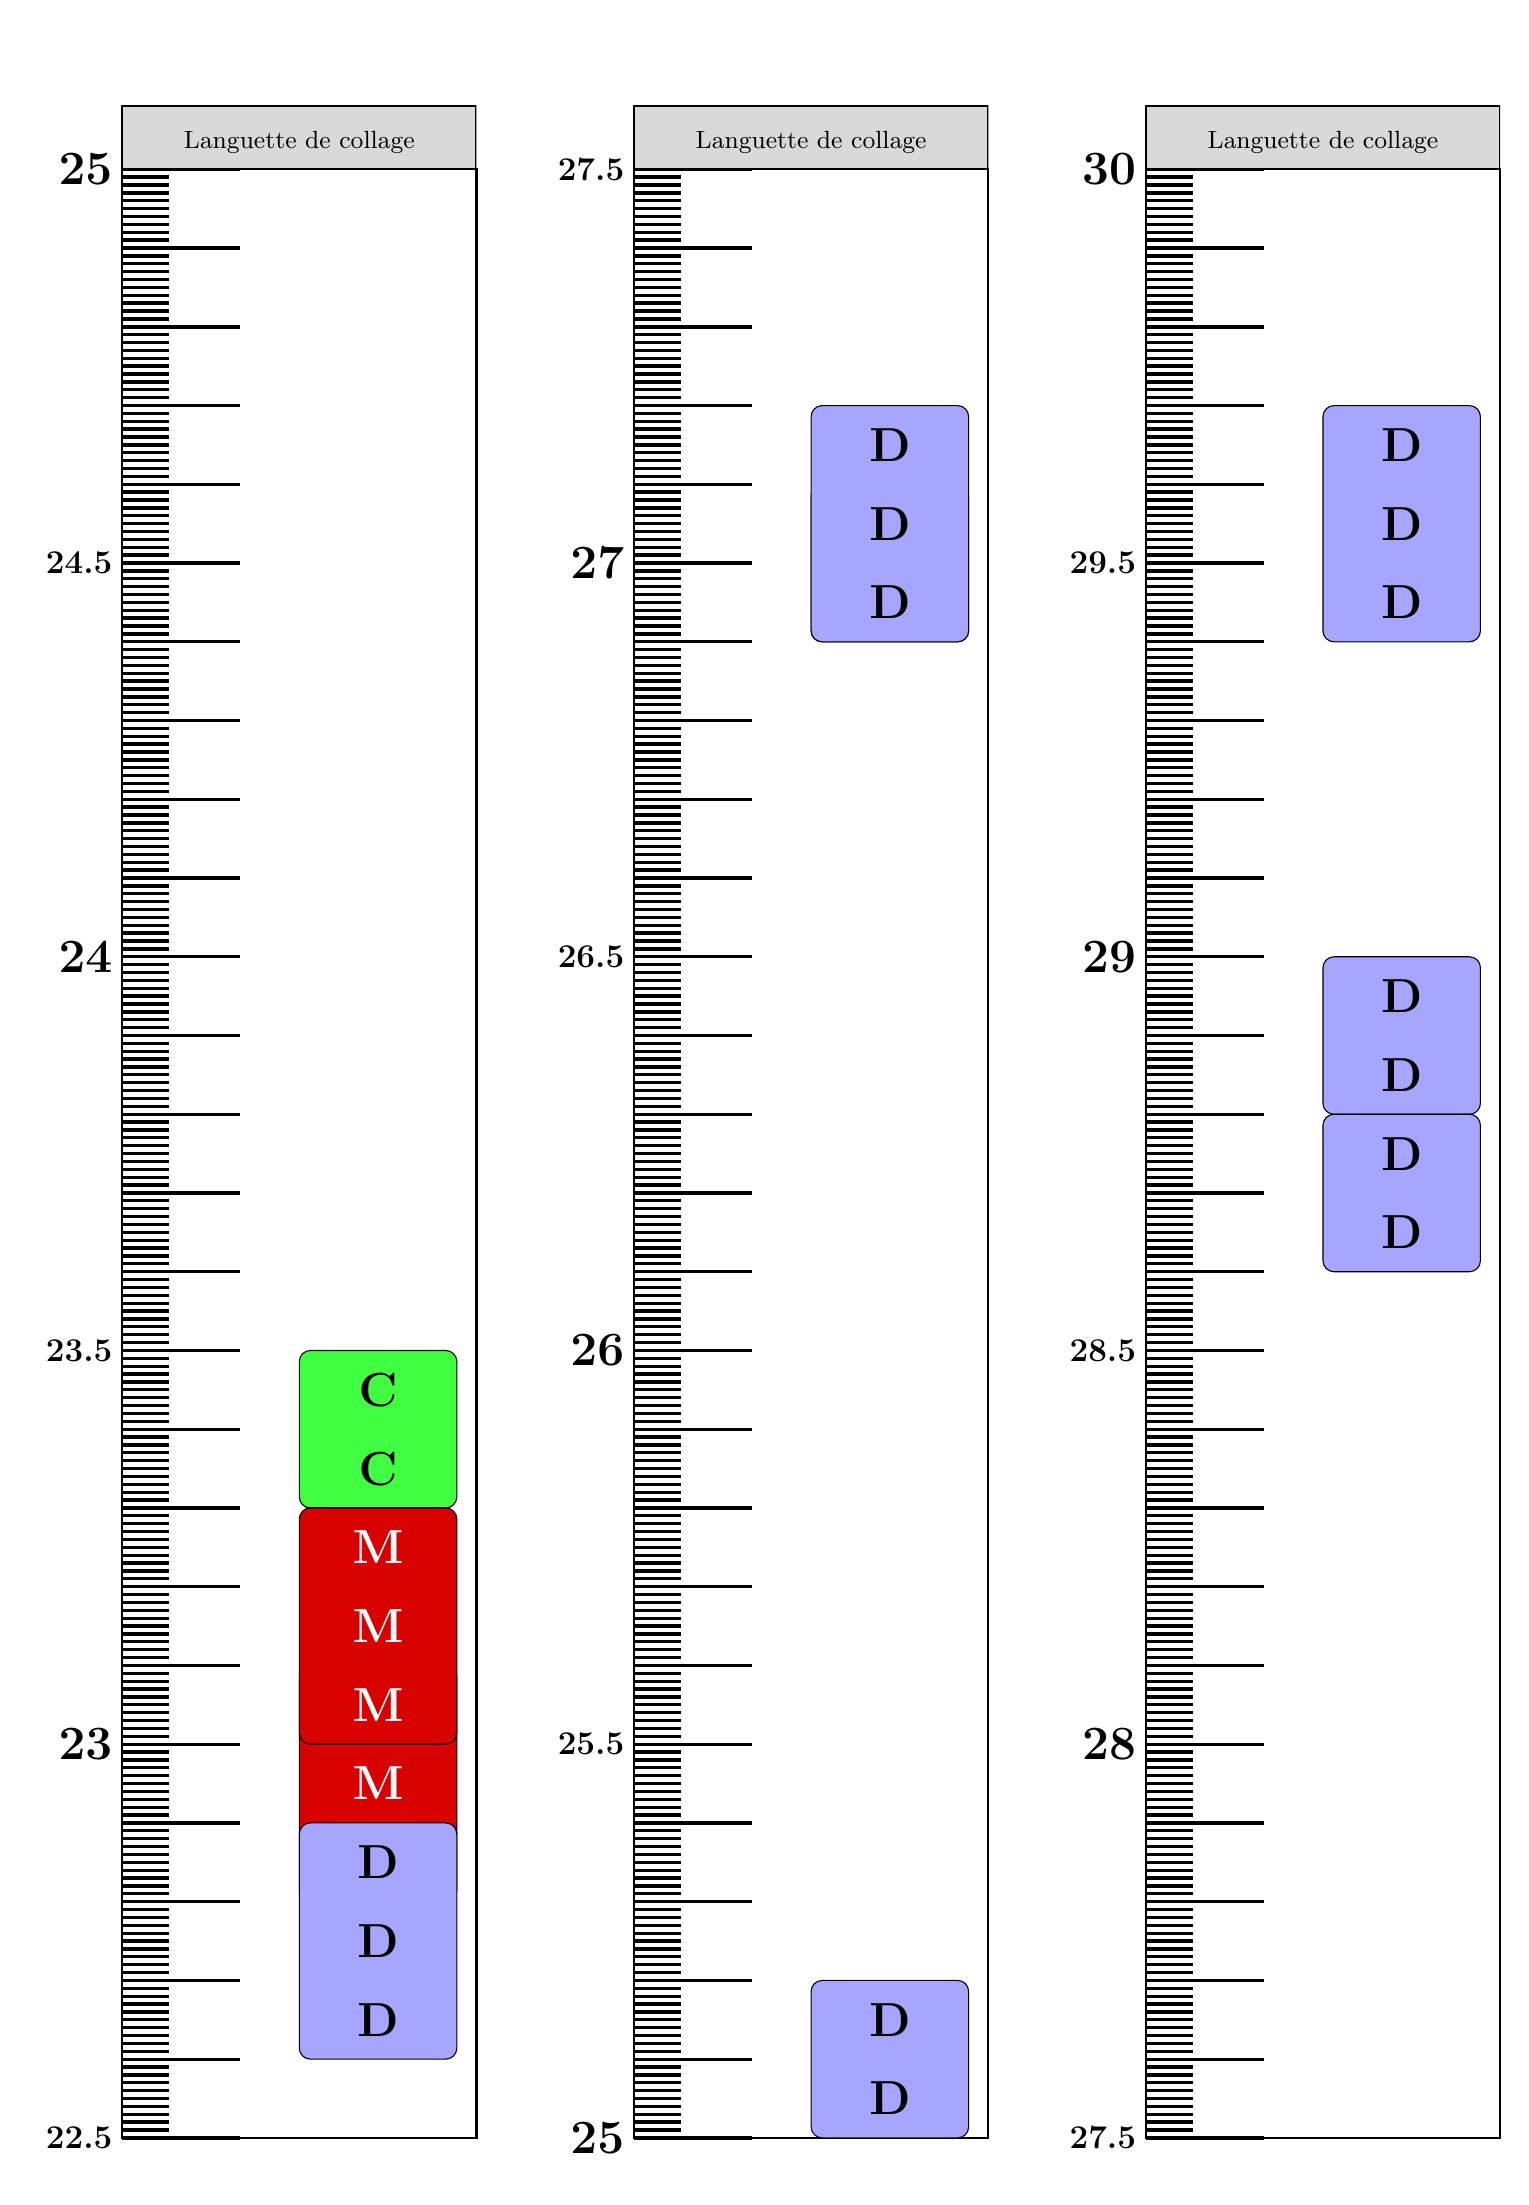
\begin{tikzpicture}[x=1cm, y=1cm,xshift=-1cm]
% Dessin de la première bande
\begin{scope}[shift={(-1,0)}]
    \draw[thick] (0,0) rectangle (\bandwidth, \bandheight);
    \clip (-1.2,-0.5) rectangle (\bandwidth, \bandheight+\languette+1);
    \drawGraduations{0}{25}{225}
\end{scope}

% Dessin de la deuxième bande (avec continuité des nombres)
\begin{scope}[shift={(1*\bandwidth + 1,0)}]
    \draw[thick] (0,0) rectangle (\bandwidth, \bandheight);
    \clip (-1.2,-0.5) rectangle (\bandwidth, \bandheight+\languette+1);
    \drawGraduations{0}{25}{250}
\end{scope}

% Dessin de la troisième bande (avec continuité des nombres)
\begin{scope}[shift={(2*\bandwidth + 3,0)}]
    \draw[thick] (0,0) rectangle (\bandwidth, \bandheight);
    \clip (-1.2,-0.5) rectangle (\bandwidth, \bandheight+\languette+1);
    \drawGraduations{0}{25}{275}
\end{scope}

\end{tikzpicture}

\newpage

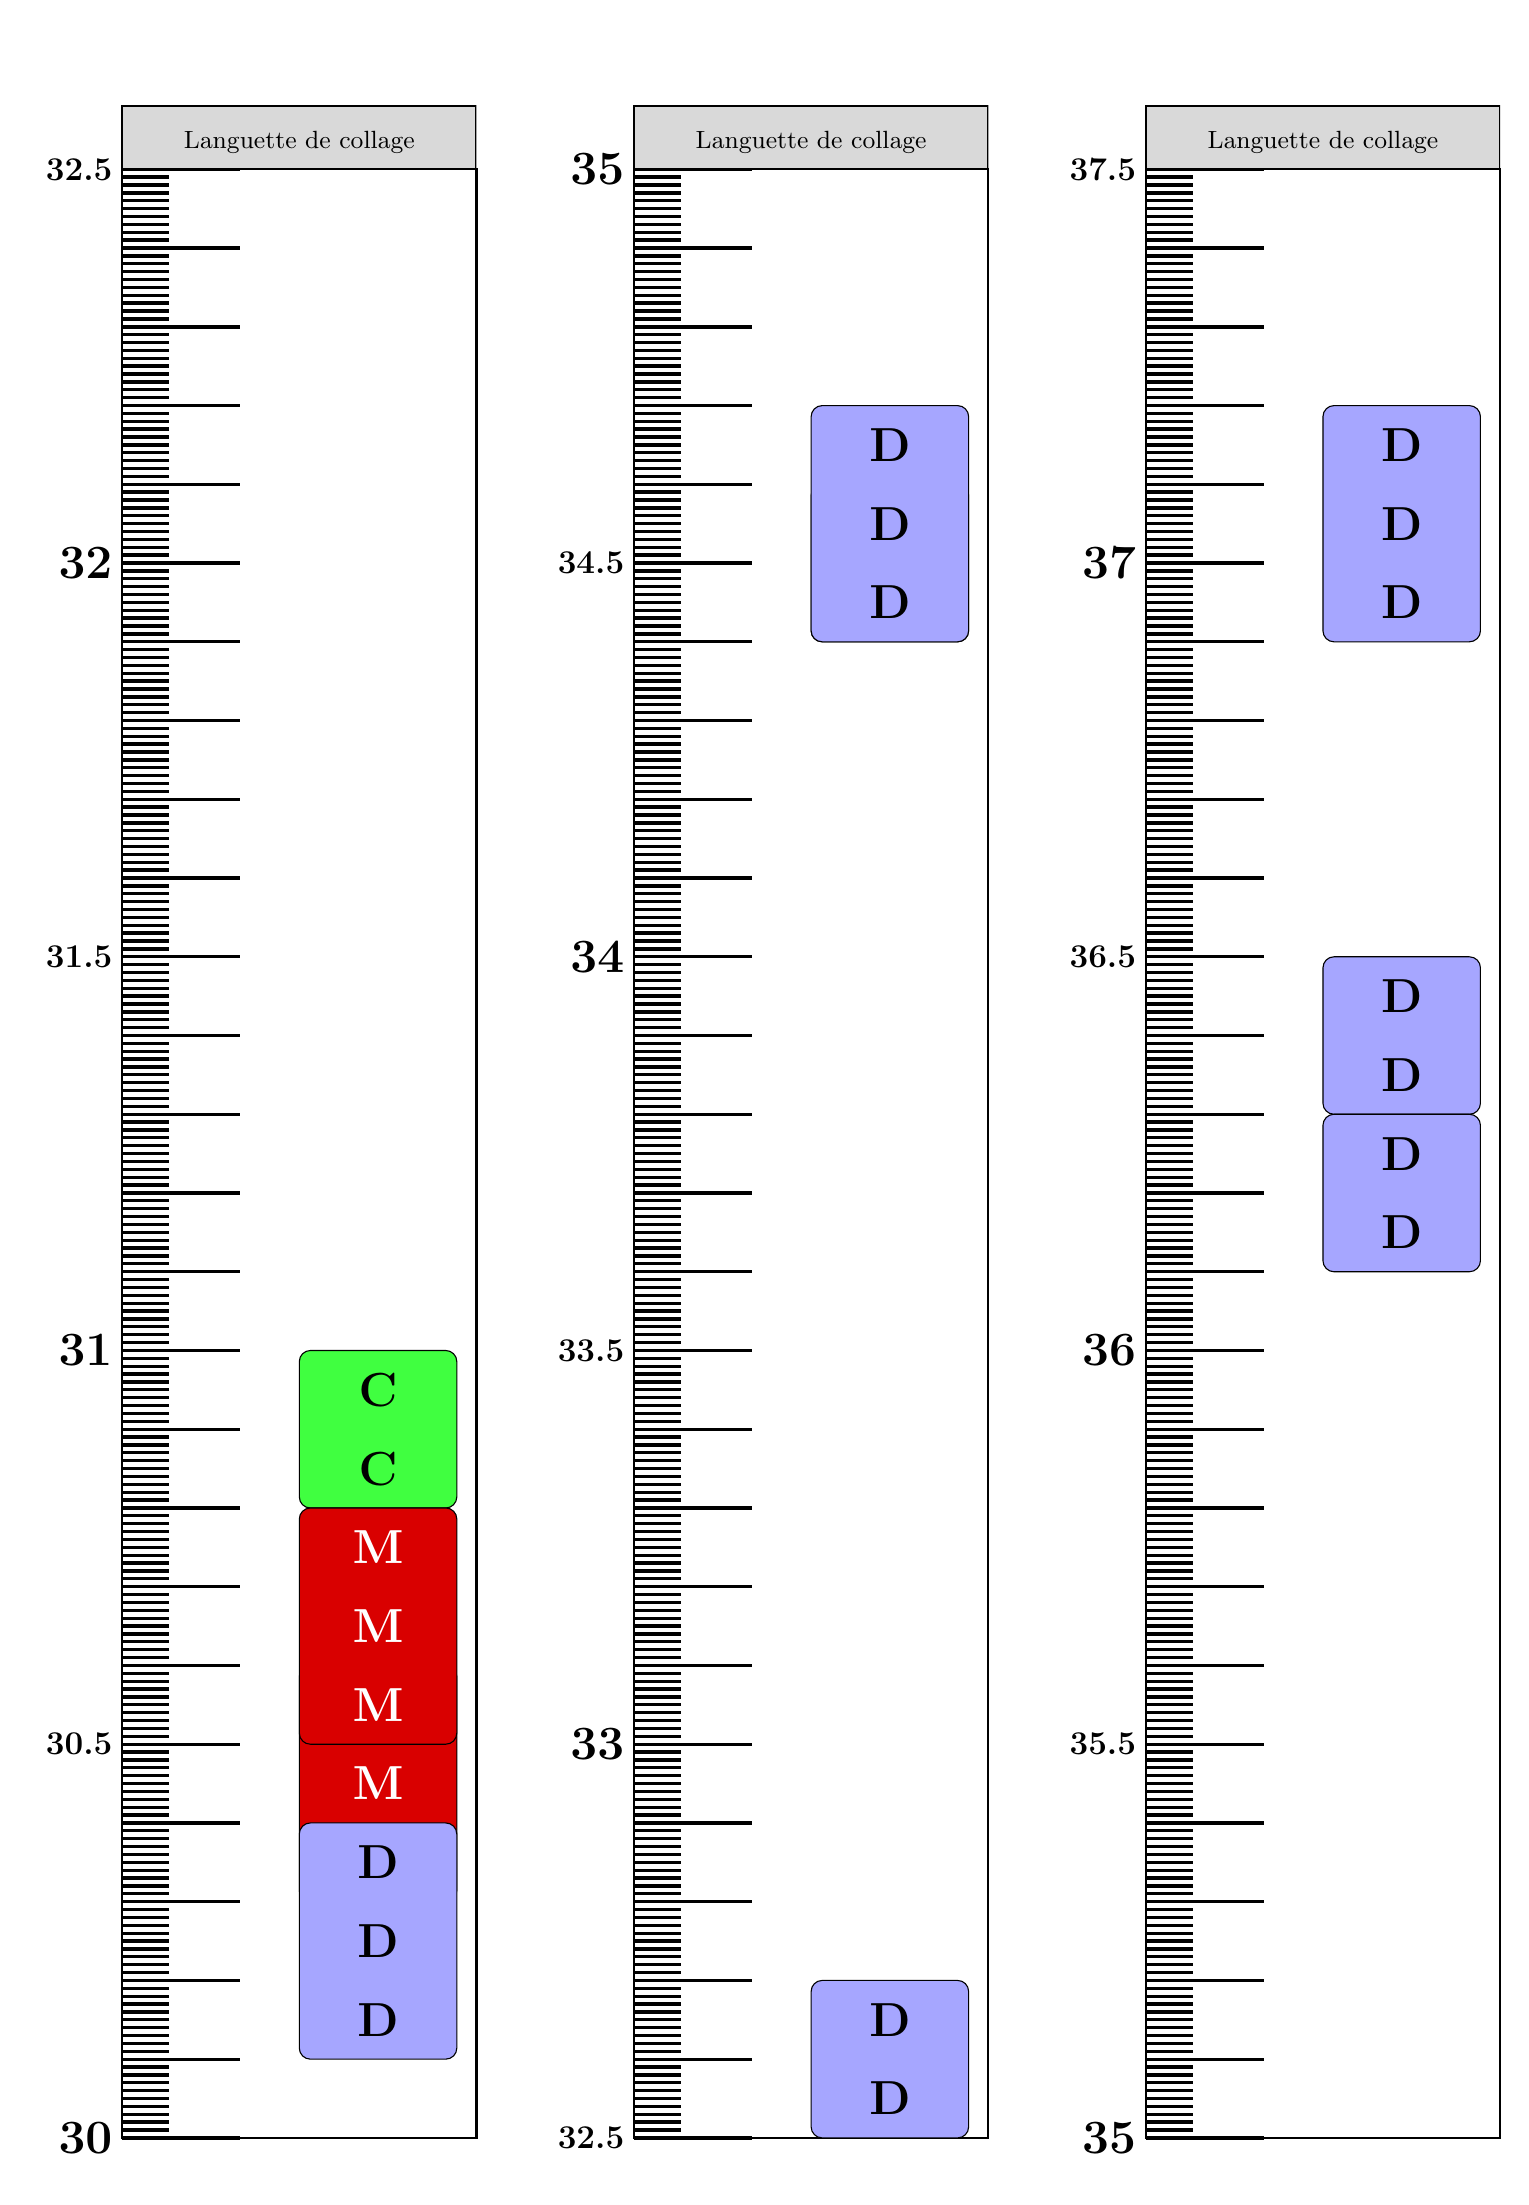
\begin{tikzpicture}[x=1cm, y=1cm,xshift=-1cm]
% Dessin de la première bande
\begin{scope}[shift={(-1,0)}]
    \draw[thick] (0,0) rectangle (\bandwidth, \bandheight);
    \clip (-1.2,-0.5) rectangle (\bandwidth, \bandheight+\languette+1);
    \drawGraduations{0}{25}{300}
\end{scope}

% Dessin de la deuxième bande (avec continuité des nombres)
\begin{scope}[shift={(1*\bandwidth + 1,0)}]
    \draw[thick] (0,0) rectangle (\bandwidth, \bandheight);
    \clip (-1.2,-0.5) rectangle (\bandwidth, \bandheight+\languette+1);
    \drawGraduations{0}{25}{325}
\end{scope}

% Dessin de la troisième bande (avec continuité des nombres)
\begin{scope}[shift={(2*\bandwidth + 3,0)}]
    \draw[thick] (0,0) rectangle (\bandwidth, \bandheight);
    \clip (-1.2,-0.5) rectangle (\bandwidth, \bandheight+\languette+1);
    \drawGraduations{0}{25}{350}
\end{scope}

\end{tikzpicture}

\newpage

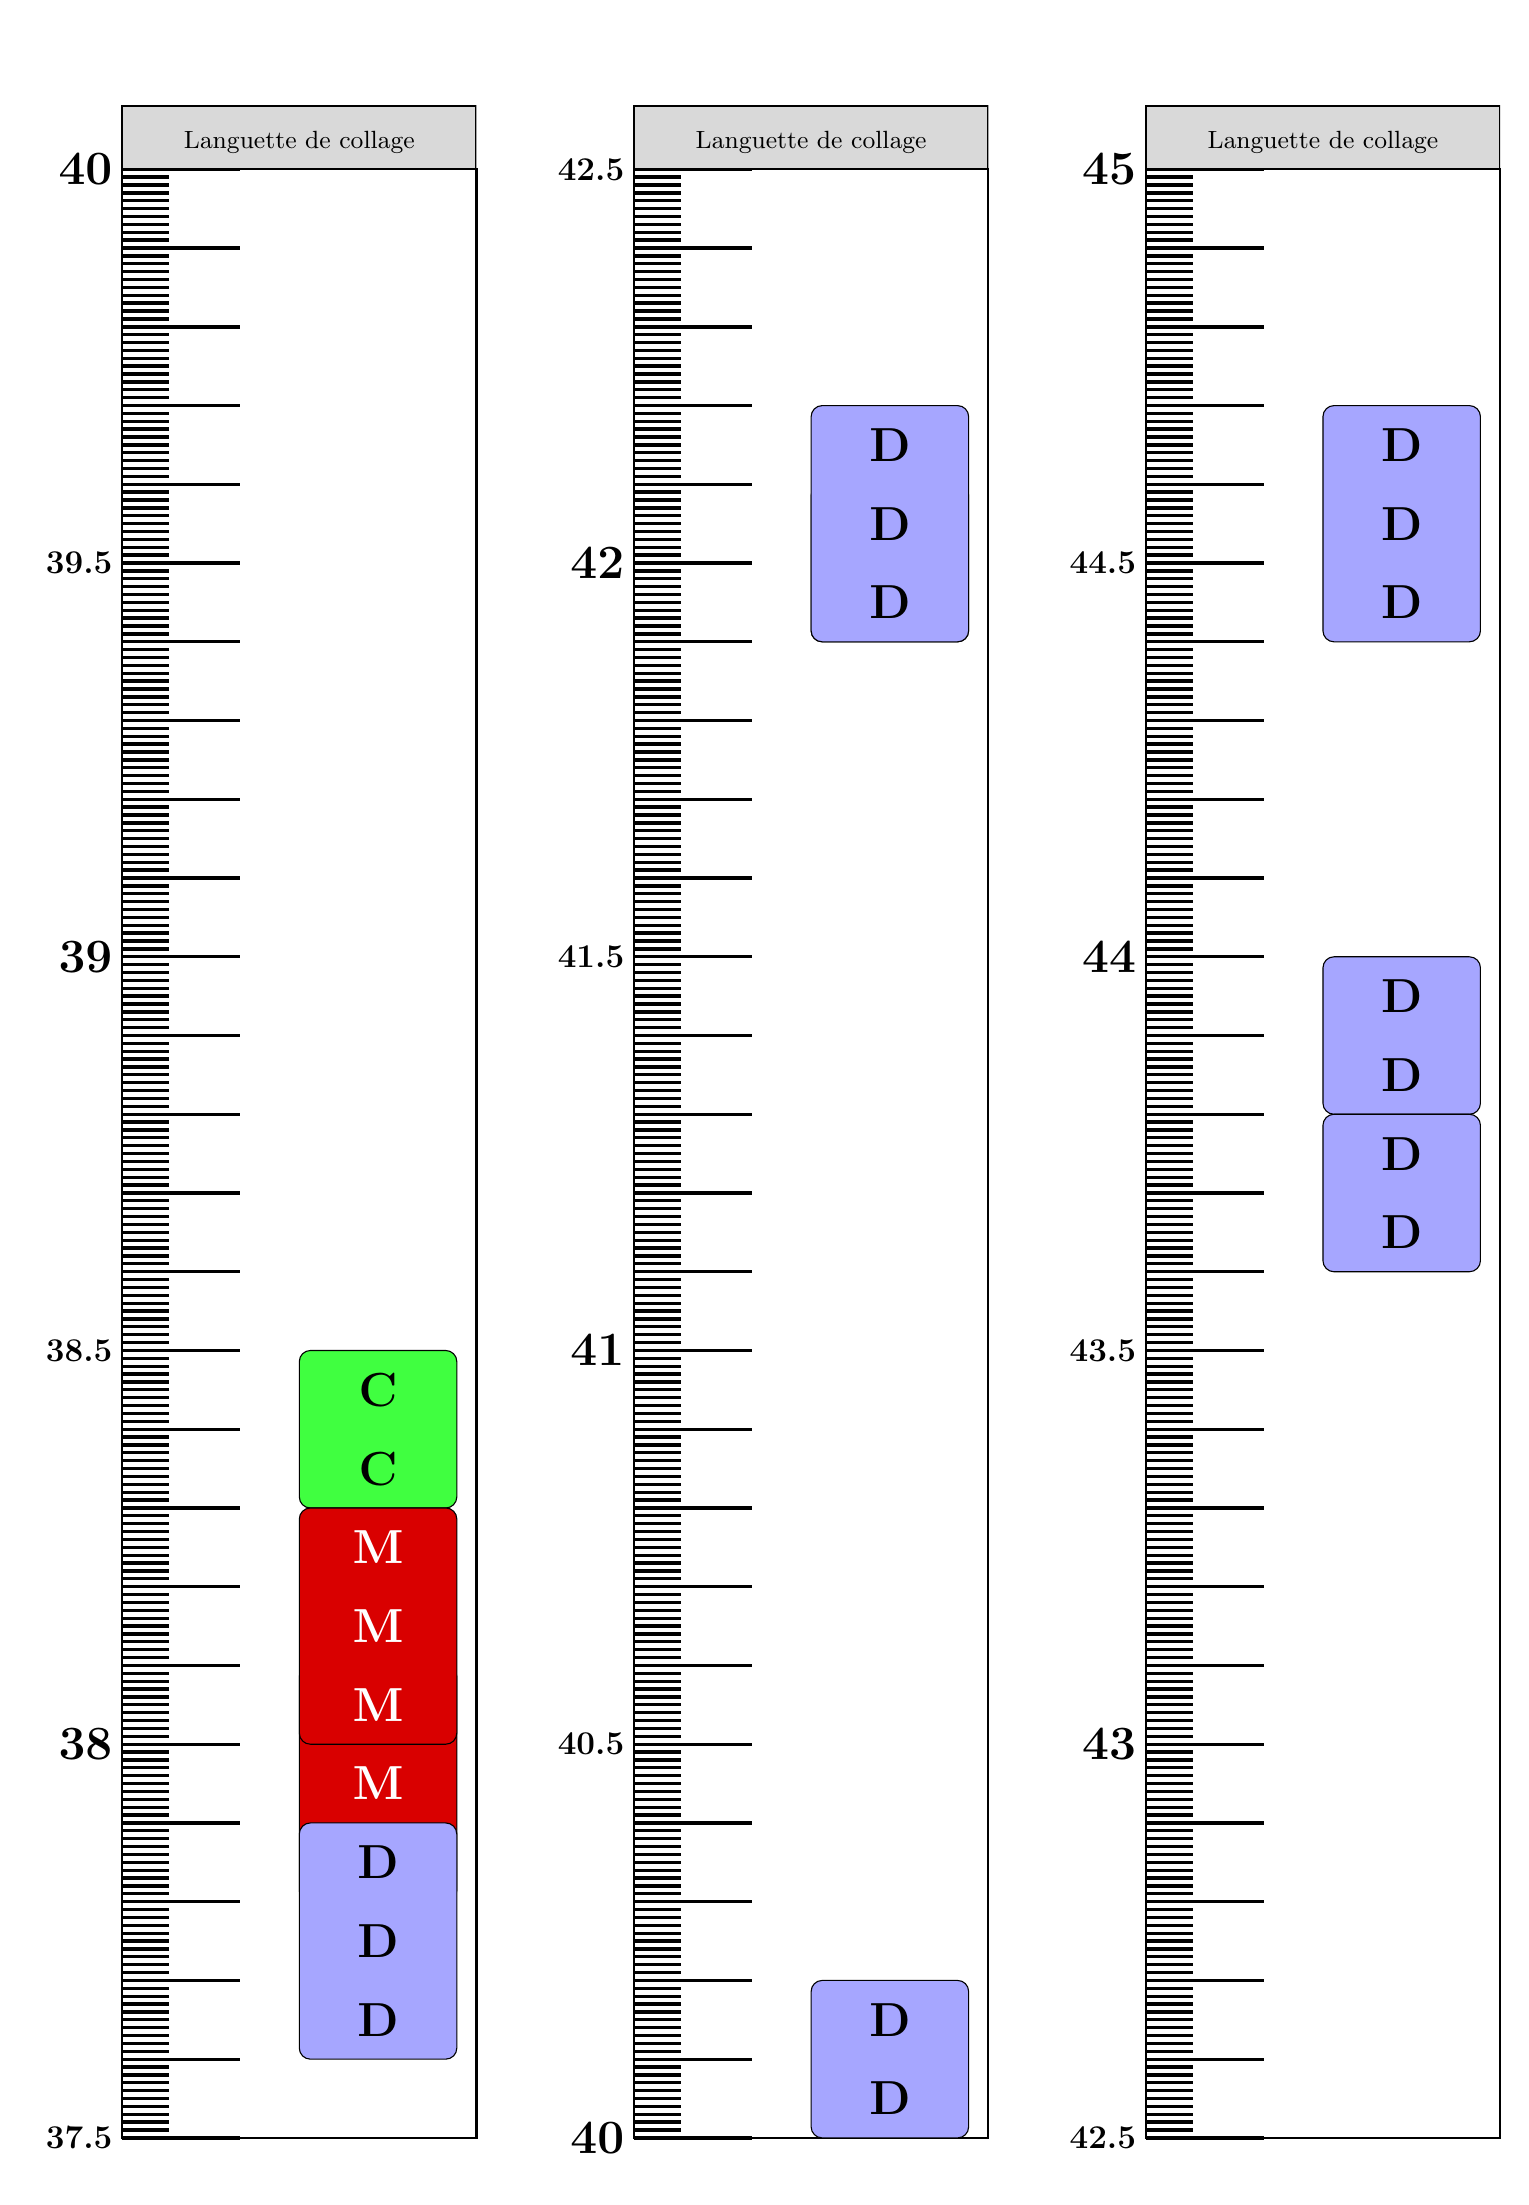
\begin{tikzpicture}[x=1cm, y=1cm,xshift=-1cm]
% Dessin de la première bande
\begin{scope}[shift={(-1,0)}]
    \draw[thick] (0,0) rectangle (\bandwidth, \bandheight);
    \clip (-1.2,-0.5) rectangle (\bandwidth, \bandheight+\languette+1);
    \drawGraduations{0}{25}{375}
\end{scope}

% Dessin de la deuxième bande (avec continuité des nombres)
\begin{scope}[shift={(1*\bandwidth + 1,0)}]
    \draw[thick] (0,0) rectangle (\bandwidth, \bandheight);
    \clip (-1.2,-0.5) rectangle (\bandwidth, \bandheight+\languette+1);
    \drawGraduations{0}{25}{400}
\end{scope}

% Dessin de la troisième bande (avec continuité des nombres)
\begin{scope}[shift={(2*\bandwidth + 3,0)}]
    \draw[thick] (0,0) rectangle (\bandwidth, \bandheight);
    \clip (-1.2,-0.5) rectangle (\bandwidth, \bandheight+\languette+1);
    \drawGraduations{0}{25}{425}
\end{scope}

\end{tikzpicture}

\newpage

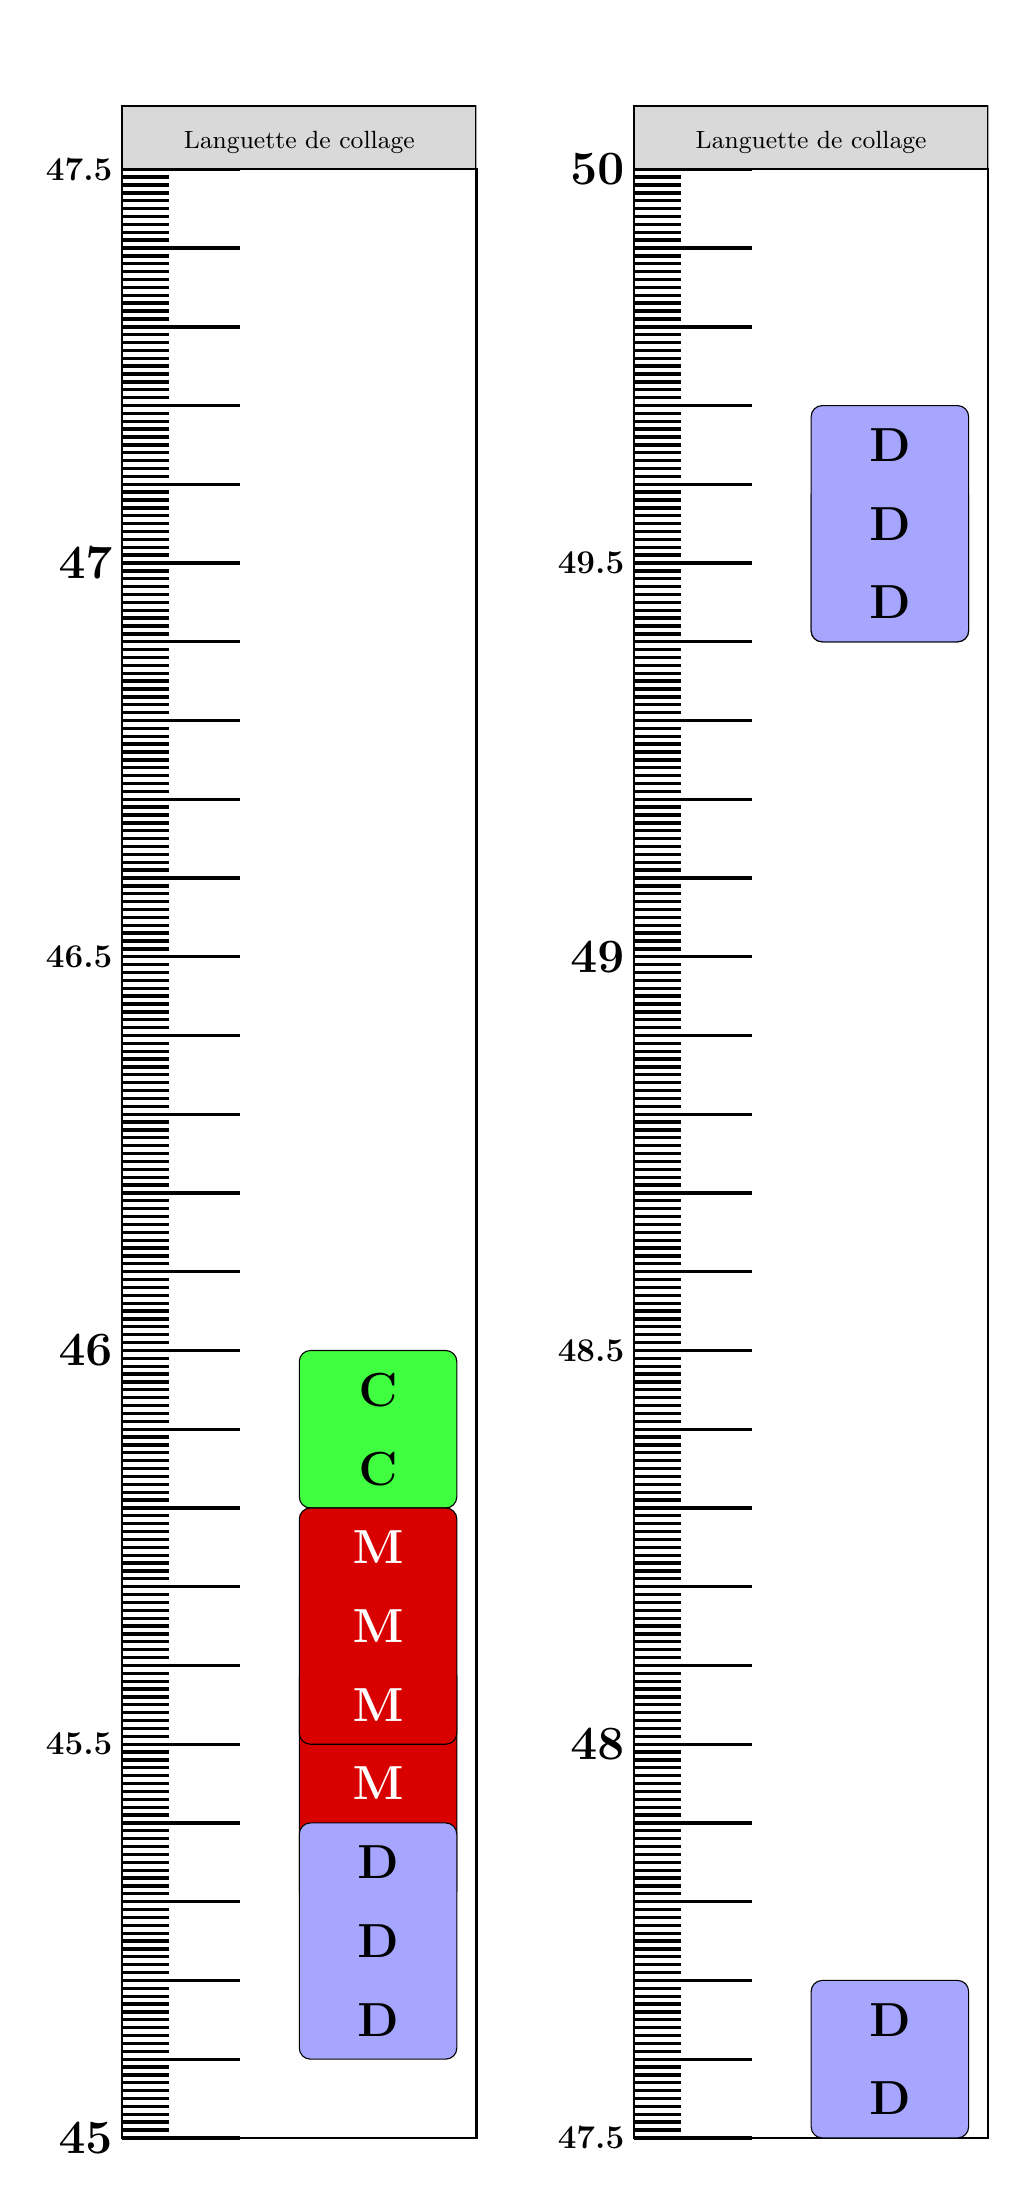
\begin{tikzpicture}[x=1cm, y=1cm,xshift=-1cm]
% Dessin de la première bande
\begin{scope}[shift={(-1,0)}]
    \draw[thick] (0,0) rectangle (\bandwidth, \bandheight);
    \clip (-1.2,-0.5) rectangle (\bandwidth, \bandheight+\languette+1);
    \drawGraduations{0}{25}{450}
\end{scope}

% Dessin de la deuxième bande (avec continuité des nombres)
\begin{scope}[shift={(1*\bandwidth + 1,0)}]
    \draw[thick] (0,0) rectangle (\bandwidth, \bandheight);
    \clip (-1.2,-0.5) rectangle (\bandwidth, \bandheight+\languette+1);
    \drawGraduations{0}{25}{475}
\end{scope}

\end{tikzpicture}
